%% ----------------------------------------------------------------
%% Thesis.tex -- MAIN FILE (the one that you compile with LaTeX)
%% ---------------------------------------------------------------- 

% Set up the document
\documentclass[a4paper, 11pt, oneside]{Thesis}  % Use the "Thesis" style, based on the ECS Thesis style by Steve Gunn
\graphicspath{Figures/}  % Location of the graphics files (set up for graphics to be in PDF format)

% Include any extra LaTeX packages required
\usepackage[square, numbers, comma, sort&compress]{natbib}  % Use the "Natbib" style for the references in the Bibliography
\usepackage{pdfpages}
\usepackage{verbatim}  % Needed for the "comment" environment to make LaTeX comments
\hypersetup{urlcolor=blue, colorlinks=true}  % Colours hyperlinks in blue, but this can be distracting if there are many links.

%% ----------------------------------------------------------------
\begin{document}
\frontmatter      % Begin Roman style (i, ii, iii, iv...) page numbering

% Set up the Title Page
\title  {Title}

\authors {Gubler Fabian}
\addresses  {\groupname\\\deptname\\\univname}  % Do not change this here, instead these must be set in the "Thesis.cls" file, please look through it instead

\maketitle
%% ----------------------------------------------------------------

\setstretch{1.3}  % It is better to have smaller font and larger line spacing than the other way round

% Define the page headers using the FancyHdr package and set up for one-sided printing
\fancyhead{}  % Clears all page headers and footers
\rhead{\thepage}  % Sets the right side header to show the page number
\lhead{}  % Clears the left side page header

\pagestyle{fancy}  % Finally, use the "fancy" page style to implement the FancyHdr headers

%% ----------------------------------------------------------------
% The "Funny Quote Page"
\pagestyle{empty}  % No headers or footers for the following pages

\null\vfill
% Now comes the "Quote(s)", written in italics
\textit{“Cyber Currencies and the blockchain have the potential to radically transform the way we think about and interact with money, and to fundamentally change the structure of our economic and social systems.”}

\begin{flushright}
Vitalik Buterin (Founder of Ethereum)
\end{flushright}

\null\vfill
\textit{Encryption will have very serious consequences for law enforcement and national security agencies at all levels. Sophisticated criminals will come to count on these means of evading detection. It’s the equivalent of a closet that can’t be opened. A safe that can’t be cracked. And my question is, at what cost?}

\begin{flushright}
James Comey (Former Director of the FBI)
\end{flushright}



\vfill\vfill\vfill\vfill\vfill\vfill\null
\clearpage  % Quote page ended, start a new page
%% ----------------------------------------------------------------

% The Abstract Page
\addtotoc{Abstract}  % Add the "Abstract" page entry to the Contents
\abstract{
\addtocontents{toc}{\vspace{1em}}  % Add a gap in the Contents, for aesthetics

Lorem Ipsum


}

\clearpage  % Abstract ended, start a new page
%% ----------------------------------------------------------------

\setstretch{1.3}  % Reset the line-spacing to 1.3 for body text (if it has changed)

\pagestyle{fancy}  %The page style headers have been "empty" all this time, now use the "fancy" headers as defined before to bring them back


%% ----------------------------------------------------------------
\lhead{\emph{Contents}}  % Set the left side page header to "Contents"
\tableofcontents  % Write out the Table of Contents



%% ----------------------------------------------------------------
\setstretch{1.5}  % Set the line spacing to 1.5, this makes the following tables easier to read
\clearpage  % Start a new page

%% ----------------------------------------------------------------
% End of the pre-able, contents and lists of things

\addtocontents{toc}{\vspace{2em}}  % Add a gap in the Contents, for aesthetics


%% ----------------------------------------------------------------
\mainmatter	  % Begin normal, numeric (1,2,3...) page numbering
\pagestyle{fancy}  % Return the page headers back to the "fancy" style

% Include the chapters of the thesis, as separate files
% Just uncomment the lines as you write the chapters


% NOTE: Must follow IMRAD Structure: Introduction, Methods, Results, and Discussion
% \input{Chapters/Chapter0} % Sample Chapter

\chapter{Introduction}
\lhead{\emph{Introduction}}  % Set the left side page header

% Cyber currencies, also known as cryptocurrencies, have gained significant attention in recent years due to their unique features and potential impact on the economy. These digital assets use cryptography for secure financial transactions and are facilitated through the use of a decentralized ledger, known as a blockchain. The anonymity and decentralized nature of cyber currencies have made them attractive to cybercriminals as a means of payment and exchange, leading to their use in a range of illicit activities such as money laundering, human trafficking, and drug trafficking (Böhme et al., 2015).

%%%%%%%%%%%%%%%%%%%%%%%%%%%%%%%%%
% Hook
%%%%%%%%%%%%%%%%%%%%%%%%%%%%%%%%%
Cyber currencies have attracted considerable attention in recent years due to their distinctive characteristics and potential economic impact. These virtual assets use cryptography to enable secure financial transactions and are facilitated through the use of a decentralized ledger, known as the blockchain. The anonymous and decentralized nature of cyber currencies has made them attractive for cybercriminals as a means of payment and exchange. In this regard, cyber currencies are facilitating a variety of illegal operations, such as money laundering, ransomware attacks, and drug trafficking \cite{bohme_bitcoin_2015} (p. 230).

%%%%%%%%%%%%%%%%%%%%%%%%%%%%%%%%%
% Relation to National Security
%%%%%%%%%%%%%%%%%%%%%%%%%%%%%%%%%
As stated in Satoshi Nakamoto's infamous white paper on bitcoin, one of the primary motivations for developing cyber currencies was to exist independently of a central authority or government \cite{nakamoto_bitcoin_nodate} (p. 4). Regardless of this intentional design decision, Bitcoin and similar currencies should not be viewed as separate from nation-states. Without a doubt, quite the contrary has been observed with regard to recent pressures to counteract its harmful influences in underground black markets and cybercrime \cite{ablon_markets_2014} (p. 4-6).

%%%%%%%%%%%%%%%%%%%%%%%%%%%%%%%%%
% State-driven Cyber Crime
%%%%%%%%%%%%%%%%%%%%%%%%%%%%%%%%%
Moreover, cyber currencies are increasingly being used to fund and support cybercrime, ranging from hacking and malware attacks to more sophisticated forms like economic espionage and sabotage \cite{reuter_information_2019} (p. 22). In particular, cyber currencies have been used as a tool in these kinds of crimes, because they provide the ability to create anonymous and untraceable transactions. 

%%%%%%%%%%%%%%%%%%%%%%%%%%%%%%%%%
\section{Research Questions}
%%%%%%%%%%%%%%%%%%%%%%%%%%%%%%%%%
The use of cyber currencies in cybercrime raises a number of critical issues and challenges that affect societies on a national and global scale. This thesis aims to address these questions through a review of relevant literature and analysis of case studies. The specific research questions for this study are: 
% TODO: Compare with Lecture Hints
\begin{enumerate}
    \item What types of cyber currencies are being used in cybercrime, and for what purposes?
    \item How are state actors involved in cybercrime, and what measures are being taken to combat them?
    \item How do state-driven actions influence the development of cyber currencies, and what are the future implications?
\end{enumerate}

%%%%%%%%%%%%%%%%%%%%%%%%%%%%%%%%%
\section{Structure of the Thesis}
%%%%%%%%%%%%%%%%%%%%%%%%%%%%%%%%%
To address these questions, the remaining chapters of this thesis are organized as follows:
% VERSION 2:2
The following chapter gives a definition of cyber currencies and a brief history of them, including the key features and traits that are unique to them. This will provide a foundational understanding for the rest of the thesis.
% VERSION 2:3 (Optional - Could merge with Ch. 2)
% In Chapter 2.2, the different types of cyber currencies used in state-sponsored cybercrime are explained, along with examples and their respective distinctions.
% VERSION 1:3
In Chapter 3, we examine how cyber currencies are used in cybercrime, including the use of specific cyber currencies.
% VERSION 1:4
Subsequently, Chapter 4 examines the measures taken by state actors to combat the use of cyber currencies in cybercrime, by looking at the challenges and examining regulatory frameworks as a potential solution.
Following, Chapter 4 investigates the measures taken by state actors to combat the use of cyber currencies in cybercrime by examining cyber currency specific challenges and discussing regulatory frameworks as a potential solution.
% VERSION 2:6
Further, Chapter 5 assesses the impact of cybercrime on the development of cyber currencies, by looking at according consequences for trust and innovation and the potential for increased regulation. 
% VERSION 2:7
Finally, Chapter 6 concludes with a summary of the study's key findings, as well as implications and suggestions for future research.


 % Introduction (Santander Task Description)

% \chapter{Background} \label{Chapter2}
\lhead{\emph{Background}}  % Set the left side page header


%%%%%%%%%%%%%%%%%%%%%%%%%%%%%%%%%
% Definition
%%%%%%%%%%%%%%%%%%%%%%%%%%%%%%%%%
Cyber currencies, also known as cryptocurrencies, are a peer-to-peer version of electronic cash that use cryptography to secure financial transactions \cite{nakamoto_bitcoin_nodate} (p. 1). They are decentralized, as they can be sent directly from one party to another without going through a financial institution, such as a bank or government. Instead, they rely on a distributed ledger technology known as a blockchain that enables transactions to be recorded and verified by a network of computers. \cite{universiti_utara_malaysia_robust_2018} (p. 24). In turn, this enables a secure and transparent transfer of value without the need for a centralized financial institution \cite{buterin_ethereum_nodate} (p. 34).

\section{History of Cyber Currencies}
%%%%%%%%%%%%%%%%%%%%%%%%%%%%%%%%%
% Early stage
%%%%%%%%%%%%%%%%%%%%%%%%%%%%%%%%%
The first digital currency, DigiCash was introduced in the late 1980s, which represented a new form of electronic money based on cryptographic protocols \cite{peters_trends_2015} (p. 4). However, it was not until the creation of Bitcoin in 2009 that cyber currencies received mainstream attention and adoption. Bitcoin was first introduced in a white paper published by an individual or group using the pseudonym Satoshi Nakamoto \cite{nakamoto_bitcoin_nodate}. The white paper, which was published shortly after the 2008 financial crisis, outlined a new system for electronic transactions in which no central authority is required to verify the validity of transactions.

One of the defining features of Bitcoin is that there are only 21 million bitcoins that can be added to the blockchain through a process called mining. As pointed out by Ethereum co-founder Vitalik Buterin, the economic scarcity means that Bitcoin is more than just a technological innovation \cite{ethereum_foundation_cryptoeconomics_2019}. He argued that Satoshi Nakamoto solved the pertinent economic incentives problem of digital currencies by creatively combining cryptography with economic assumptions through the limited supply of bitcoin.

% Reflected in the trading volume / economic interest
% OPTIONAL: Graph of price movement since inception
% Source: Authors using data from Blockchain.info and Quandl.com.

%%%%%%%%%%%%%%%%%%%%%%%%%%%%%%%%%
% Other crypto
%%%%%%%%%%%%%%%%%%%%%%%%%%%%%%%%%
Since the inception of Bitcoin, a number of new cyber currencies have emerged, each with its own set of distinct attributes. Some examples include Ethereum, which pioneered the concept of smart contracts; Monero, which prioritizes privacy and anonymity; and Litecoin, which aims to be a faster and more efficient version of Bitcoin. 

The rise of cyber currencies has been met with both enthusiasm and skepticism. Proponents argue that digital assets have the potential to revolutionize the financial industry by providing a more secure and efficient means of conducting transactions \cite{lu_blockchain_2019} (p. 83). Critics, on the other hand, have expressed concern about the potential use of cyber currencies in illicit activities, negative implications for the environment as well as the lack of regulatory oversight \cite{bohme_bitcoin_2015} (p. 214).

%%%%%%%%%%%%%%%%%%%%%%%%%%%%%%%%%
\section{Key Characteristics of Cyber Currencies} \label{2.1}
%%%%%%%%%%%%%%%%%%%%%%%%%%%%%%%%%
Despite the uncertainties involving cyber currencies, it is clear that they are affecting governments and societies in many groundbreaking ways. Cyber currencies have unique characteristics that distinguish them from traditional fiat currencies and pose new challenges for nation states at large. The following characteristics are especially to be taken into account for the rest of this thesis:

\begin{itemize}
    \item \textbf{Decentralization}: Cyber currencies are not controlled by central authority and consequently operate outside the purview of traditional central banks and financial institutions. Because of the decentralized nature, it is more difficult for law enforcement agencies to track and trace the origin and destination of cyber currency transactions. Furthermore, because there is no central authority that can block or interfere with transactions, decentralization provides greater resistance to censorship.
    \item \textbf{Anonymity}: Cyber currencies offer a high degree of anonymity, as direct personally identifiable information is omitted from any transaction \cite{ober_structure_2013} (p. 237). Because of the anonymity afforded by cyber currency transactions, it has become a popular method of payment and exchange for illegal activities such as ransomware extortion and DDoS attacks \cite{noauthor_internet_nodate} (p. 11). This characteristic makes it difficult for law enforcement to track down and prosecute criminals, as well as to attribute crimes to specific individuals, groups, or nation states.
    \item \textbf{Lack of regulation:} In many cases, cyber currencies are not subject to the same regulations and oversight as traditional financial systems. Furthermore, the rapid growth and increasing mainstream adoption of cyber currencies has led to a number of geopolitical tensions. Individual nations adopt different approaches when it comes to regulating and taxing cyber currency transactions \cite{law_at_sogang_university_school_of_law_jd_pittsburgh_current_2021} (p. 146).
\end{itemize}

% TODO: Check if all is covered
Given the decentralized, anonymous, and largely unregulated nature of cyber currencies, it is not surprising that cyber currencies have become a popular means of exchange in the world of cybercrime. Before delving into the role of state actors and their impact involving cybercrime, we must in the following chapter examine the various ways in which cyber currencies are used in cybercrime. % Methods
%
% \chapter{Use of Cyber Currencies in Cyber Crime}
\lhead{\emph{Use of Cyber Currencies in Cyber Crime}}  % Set the left side page header

Cyber currencies, have been used to facilitate the sale of illegal goods and services. Although these transactions can be done using non-digital currencies, illicit sites are increasingly moving toward accepting only digital cyber currencies, because they enforce anonymity and security features \cite{ablon_markets_2014} (p. 11). 

The majority of illicit transactions are taking place on the dark web. This is due to its web architecture enhancing the security and encryption capabilities of its users, further enhancing the anonymity characteristics of cyber currencies. \cite{ablon_markets_2014}. The dark web contains content that has been intentionally concealed, typically including illegal and anti-social information, which "can only be accessed through specialized browsers such as Tor (short for The Onion Router)" \cite{weimann_going_2016} (p. 196).

\section{Overview of Cyber Currencies}

\subsection*{Bitcoin}
Bitcoin is the most widely used cyber currency in the sale of illegal drugs \cite{kim_get_2022} (p. 1). As the foremost and most well-known cyber currency, Bitcoin has a large user base and is accepted by a wide range of merchants, including those on the dark web. This makes it a convenient choice for individuals and organizations involved in illegal activities. In particular, Bitcoin as a currency is easily acquired, used, and exchanged, such as through the use of a Bitcoin ATM \cite{irwin_use_2016} (p. 414).

\subsection*{Monero}
Monero, a privacy-focused currency, is another cyber currency that has been used in black markets. Monero protects its users' confidentiality by employing advanced cryptographic techniques such as stealth addresses and ring signatures \cite{averin_review_2020} (p. 83). Regarding criminal activity, it has become a popular choice for ransomware attacks, because cybercriminals can demand payments in Monero without the risk of being traced.

\subsection*{Zcash}
Zcash is another cyber currency that is used in black markets and is often referred to as a more privacy-focused alternative to bitcoin. It is based on the same underlying technology as Bitcoin, but adds features that allow users to keep their transaction details private, by using a cryptographic technique called Zero Knowledge Proof \cite{harikrishnan_secure_2019} (p. 307). This makes Zcash especially appealing for use on the dark web. As a result, in instances where anonymity and privacy are essential, some marketplaces may even only accept Zcash as a payment method.

\subsection*{Implications for cybercrime}
It follows that cyber currencies, the dark web, and illegal activities are inextricably linked. More specifically, the anonymity and decentralization of cyber currencies make them ideal for the dark web, allowing users to conduct transactions without revealing their identities or leaving a traceable financial trail. More concretely, the anonymity and decentralization of cyber currencies make them a perfect fit for the dark web, as they allow users to make transactions without revealing their identities or leaving a traceable financial trail. Overall, Bitcoin is a popular choice for black market transactions due to its relative stability and liquidity compared to other cyber currencies. However, there is no agreement on which type of cyber currency is to be seen as the clear leader, as many currencies are interchangeable \cite{ablon_markets_2014} (p. 12).

\section{Types of Illegal activities}
There exists a number of ways in which cyber currencies are used to facilitate illegal activities. The following section concentrates on three major types of illegal activities that are closely related to cyber currencies: illicit drug sales, money laundering, and ransomware attacks. 

Throughout the section, a series of cases are presented to demonstrate how these activities are carried out using cyber currencies. These case studies will provide concrete examples of how cyber currencies are used in each of these illegal activities, allowing us to gain a better understanding of the motivations and mechanisms behind them. 

\subsection*{Illicit drug sales}

Cyber currencies are the primary form of payment on the dark web and have been used to facilitate the sale of illegal drugs. The Silk Road marketplace is one prominent example of illicit drug sales taking place on the dark web. The Federal Bureau of Investigation (FBI) shut down Silk Road in 2013, and its founder, Ross Ulbricht, was sentenced to life in prison. \cite{dolliver_evaluating_2015} (p. 1113).  According to the FBI's criminal complaint filed in the trial of Ross Ulbricht, the Silk Road market had nearly 150,000 buyers and nearly 4,000 vendors \cite{noauthor_united_nodate}. Despite its clearly unlawful operations, Silk Road provided an appealing value proposition to its users in the form of a close-knit community focused on the reliability of vendors and safe drug use \cite{lacson_21st_2016} (p. 46). One user, for example, stated that “relationships between vendors and consumers were based on levels of trust and professionalism” \cite{van_hout_silk_2013} (p. 387).

Regardless of this high-profile takedown, the use of cyber currencies in the sale of illegal drugs has continued to thrive on other dark web marketplaces. To illustrate, only two years later, the dark net aggregator DNStats.net listed 22 new Dark Net markets. Over 46,000 drugs were listed for sale on these markets, compared to 18,000 in October 2013, when Silk Road was shut down \cite{digital_citizens_alliance_silk_2015}. Moreover, it is expected that activity on the dark web and the use of cyber currencies will further increase in the coming years \cite{ablon_markets_2014} (p. 31).

\subsection*{Money Laundering}

Cyber currencies are frequently used to disguise the proceeds of illegal activities as legitimate funds, a process known as money laundering. Because cyber currencies are decentralized and barely regulated by any government or financial institution, they are an appealing vehicle used in money laundering.

Despite advancements in methods by which government institutions can reduce the ability to launder money, many mechanisms that provide anonymity continue to exist \cite{dupuis_money_2020} (p. 61). These “open door” technologies and products make it difficult for law enforcement to track and trace transactions involving cyber currencies. Additionally, the use of cyber currencies allows individuals to transfer funds across borders without going through traditional financial institutions \cite{filipkowski_cyber_2008} (p. 17), making money laundering even more difficult to detect and prevent.

There have been several cases where nation states have used cyber currencies to launder money and avoid economic sanctions. Venezuela, for instance, was sanctioned economically by the Trump Administration in 2018 for money laundering. These sanctions targeted the use of the country's own government-issued cyber currency, "Petro". \cite{noauthor_radical_nodate} (p. 1325). Petro emerged as an opportunity to raise new funds for the government and bypass US sanctions. It aspired to circumvent the existing barriers between Venezuelan financial operations and companies of the United States \cite{uzcategui_versatile_2020} (p. 193).

% Bonus: The case of Iran: In 2020, the U.S. Department of the Treasury's OFAC imposed economic sanctions on Iran and targeted the country's use of cryptocurrencies for money laundering and sanctions evasion. According to OFAC, Iran was using cryptocurrencies to "bypass U.S. economic sanctions and access the international financial system."

%%%%%%%%%%%%%%%%%%%%%%%%%%%%%%
% Bonus: ATMS
%%%%%%%%%%%%%%%%%%%%%%%%%%%%%%
% Another reason cyber currencies are used in money laundering is that they can be easily converted“open door”currency, such as US dollars or euros, through exchanges. This allows individuals to convert their illicit funds into a more widely accepted and usable form of currency.
  
% An example of this  is the use of cryptocurrency ATMs to launder money. According to a report published by Europol, "cryptocurrency ATMs are increasingly being used by money“launderers to convert illicit cash into virtual currency and vice versa." The report goes on to state that "criminals are attracted to the anonymity and lack of regulation of cryptocurrency ATMs, which makes them an attractive means of laundering illicit proceeds."

\subsection*{Ransomware Attacks}
Ransomware is a special type of malware which aims to encrypt a victim's files using strong
cryptography and demands a ransom from the victim to restore access to the files \cite{gonzalez_detection_2017} (p. 472).  Cybercriminals often demand payment in cyber currencies, in exchange for the decryption key to unlock the encrypted data.

The use of cyber currencies in ransomware attacks has enabled perpetrators to demand ransom payments in a difficult to trace manner, causing significant disruptions and financial losses for affected victims. Cyber currencies, such as Bitcoin, Monero, and Zcash, have had a significant impact on the proliferation of ransomware attacks. In 2021 alone, North America saw a 180 percent increase in ransomware attacks, while Europe saw an increase of 234 percent \cite{sonicwall_mid-year_2021} (p. 9). At the same time, the effective payments of ransomware attacks has risen significantly. In this case, up from 34 percent paid in 2020, 58 percent of ransomware-infected organizations agreed to pay a ransom in 2021 \cite{proofpoin”_2022_2022} (p.47).

One high-profile example of ransomware attacks is the WannaCry attack that occurred in May 2017. This cyberattack is considered the largest ransomware outbreak in history, impacting over 200,000 computers in 150 countries, extorting a relatively small sum of USD 140,000 in Bitcoin \cite{alraddadi_comprehensive_nodate} (p. 1, 5).

\subsection*{Other activities}
It is important to note that the use of cyber currencies for illegal purposes is not limited to these three activities. Cyber currencies also facilitate other types of illegal activity, such as fraud, cyber-enabled theft, and human trafficking. In addition, aside from black markets, cyber currencies, such as Bitcoin and others, have been used in a number of investment scams. These scams frequently involve deceptive investment schemes in which individuals are promised high returns in exchange for investing in virtual currencies. It is also worth noting  that while cyber currencies can be used to facilitate illegal activities, they are not inherently illegal and can also be used for legitimate purposes. Overall, because these transactions are anonymous, it can be difficult for law enforcement to track down and prosecute individuals involved in illegal activities.  % Data
%
% \chapter{Approaches to Combat Illicit Use of Cyber Currencies}
\lhead{\emph{Approaches to Combatting the Illicit Use of Cyber Currencies}}  % Set the left side page header

%%%%%%%%%%%%%%%%%%%%%%%%%%%%%%%
\section{Challenges for Law Enforcement Agencies}
%%%%%%%%%%%%%%%%%%%%%%%%%%%%%%%

The anonymity of cyber currency transactions on the dark web makes it a popular choice for criminal activities, as it allows individuals and organizations to operate with a degree of protection from law enforcement. This anonymity, however, makes it difficult for authorities to track down and prosecute those engaged in illegal activities on the Dark Web. Furthermore, searching for criminal activity becomes an ongoing challenge for law enforcement because most search engines can only query results from the Clearnet \cite{lacson_21st_2016} (p. 45) \cite{zheng_learning_2013} (p. 201). 

To address these issues, law enforcement agencies have put in place a variety of measures, including the use of specialized software to track down cyber currency transactions. In addition, law enforcement is forming alliances with cybersecurity experts and other agencies to broaden their knowledge and expertise \cite{europol_internet_2017} (p. 40). However, due to the rapid evolution of cyber currencies and the sophisticated tactics used by cybercriminals, law enforcement agencies have found it difficult to keep up with the evolving threat. Concerning this issue, Christin suggested a number of ways to combat criminal activity on the dark web and has proposed "four intervention strategies that could be considered: disrupting the network, disrupting the financial infrastructure, disrupting the delivery model, and laissez-faire \cite{christin_traveling_2013} (p. 220).

The first option would involve shutting down the Tor network. This is nearly impossible because any computer with Tor installed can act as a node, with the software operating on a global scale. To put it differently, while a court order in one country may shut down a few nodes, removing a significant portion of nodes would require multinational cooperation \cite{dingledine_design_2006} (p. 4). 
The second option refers to the financial infrastructure of cyber currencies such as Bitcoin. This would involve an "attempt to manipulate the currency to create rapid fluctuations and impede transactions" \cite{christin_traveling_2013} (p. 221). While this is more feasible than stopping Tor, it would require significant financial investment and would most likely only be a temporary solution \cite{lacson_21st_2016} (p. 45). 
Third, another possible attack strategy is to disrupt the delivery model of illegal goods. That is, to strengthen controls at the post office and at customs to prevent illegal items from reaching their destination \cite{christin_traveling_2013} (p. 222). Finally, one last possible intervention strategy is to not intervene at all. Despite the fact that this is a politically questionable proposition, studies for instance show that preventing drug abuse is a far more cost-effective than enforcing drug prohibition \cite{christin_traveling_2013} (p. 222).

%%%%%%%%%%%%%%%%%%%%%%%%%%%%%%%
\section{Regulatory Frameworks}
%%%%%%%%%%%%%%%%%%%%%%%%%%%%%%%
As a whole, it was demonstrated that governmental law enforcement agencies have a number of options for combating the use of cyber currencies in cybercrime. Another approach has been to implement regulatory frameworks aimed at preventing illicit cyber currency  use in order to increase transparency in cyber currency transactions. These frameworks vary by country and take very different approaches. Some regulators may place an emphasis on consumer protection, while others focus on financial safety and integrity. \cite{narain_aditya_regulating_2022}. 

The Financial Action Task Force (FATF) recommendations is a prominent example of a widely accepted regulatory framework. Over 180 countries have endorsed the FATF recommendations \cite{financial_action_task_force_fatf_2012} (p. 7), which are universally recognized as the international standard for anti-money laundering efforts and countering the financing of terrorism. FATF moved quickly to provide a global framework for the regulation of virtual assets, including cyber currencies. These recommendations include provisions for the regulation of virtual asset service providers (VASPs), such as exchanges and wallet providers \cite{financial_action_task_force_fatf_2012} (p. 76). These in turn must put in place safeguards to ensure customer due diligence, record-keeping, and reporting of suspicious activity.

Besides the FATF recommendations, there are a number of other regulatory frameworks that address cyber currency use. These may include national laws and regulations, as well as international agreements. Some countries (including Japan and Switzerland) have amended or introduced new legislation governing cyber assets and service providers, while others (including the European Union, the United Arab Emirates, the United Kingdom, and the United States) are at the drafting stage \cite{narain_aditya_regulating_2022}. 

\section{Feasibility of Regulation}
In general, regulating cyber currency and virtual assets is a complicated and changing field. State actors are trying to find a balance between the possible benefits of these technologies and the need to stop them from being used illegally. The implementation of regulatory frameworks has received both praise and criticism. Supporters argue that these measures are necessary to protect consumers from fraud and to ensure the integrity of the financial system \cite{financial_action_task_force_fatf_2012} (p. 9). Critics, on the other hand, have expressed concern about regulatory frameworks' potential to stifle innovation and the growth of cyber currencies \cite{demertzis_economic_2018} (p. 10).

Furthermore, the feasibility of regulatory measures informs a secondary debate about legal ethics. Internet freedom has been fought for in courts since its inception. This due to it being a bastion of free speech and a tool for great good and innovation in the world  \cite{lacson_21st_2016} (p. 45). Andrew argues that when it comes to internet freedom, "it is impossible not to feel that any policing is regrettable"  \cite{andrew_internet_2010} (p. 1098). One such example is that while cyber currencies facilitate illegal activities, they also provide many liberties to people living under oppressive regimes by allowing them true anonymity.

%%%%%%%%%%%%%%%%%%%%%%%%%%%%%%%
% National Cyber Currencies
%%%%%%%%%%%%%%%%%%%%%%%%%%%%%%%

% Another approach has been the creation of national cryptocurrencies, which are digital currencies issued and backed by a national government. These currencies can be used as an alternative to traditional fiat currencies and may offer benefits such as increased speed and efficiency in financial transactions, as well as enhanced security. However, the use of national cryptocurrencies also raises concerns about centralization and the potential for governments to exert greater control over their citizens' financial activities.

% In addition to regulatory frameworks, some state actors have also developed national cyber currencies, which are digital assets issued and backed by the government (Central Bank of China, 2020). National cyber currencies are designed to provide a secure and transparent means of conducting financial transactions, while also allowing for the tracking and tracing of transactions to ensure compliance with relevant laws and regulations (Central Bank of China, 2020).

% The development of national cyber currencies has been met with both support and criticism. Supporters argue that these digital assets have the potential to provide a more secure and efficient means of conducting transactions and reduce the risk of cyber crime (Central Bank of China, 2020). Critics, on the other hand, have raised concerns about the potential for national cyber currencies to be used for surveillance and control (Buterin, 2014).

%%%%%%%%%%%%%%%%%%%%%%%%%%%%%%%
% \section{Effectiveness of Measures}
%%%%%%%%%%%%%%%%%%%%%%%%%%%%%%%

%%%%%%%%%%%%%%%%%%%%%%%%%%%%%%%%%%%%%
% State-driven
%%%%%%%%%%%%%%%%%%%%%%%%%%%%%%%%%%%%%

% State-driven cyber crime poses significant challenges and risks, including the potential for damage to international relations and the reputational consequences of these crimes. In response, a number of measures have been taken by law enforcement and regulatory agencies to combat this type of crime.

% One approach has been the use of law enforcement efforts to track and seize cyber currency funds that have been obtained through illicit means. For example, the U.S. Department of Justice has established a Cybercrime Unit specifically dedicated to investigating and prosecuting cyber crimes, including those involving cyber currencies (U.S. Department of Justice, n.d.). In addition, the U.S. Secret Service has a dedicated Cyber Intelligence Section that focuses on tracking and disrupting cyber crime, including the use of cyber currencies (U.S. Secret Service, n.d.).

% Another approach has been the implementation of regulations and laws to combat cyber crime, including state-driven cyber crime. For example, the U.S. has implemented the Bank Secrecy Act, which requires financial institutions to report suspicious activity, including the use of cyber currencies, to the Financial Crimes Enforcement Network (FINCEN) (U.S. Department of the Treasury, n.d.). In addition, the U.S. has implemented the Travel Rule, which requires financial institutions to report information about the sender and recipient of cross-border transactions over $3,000 (U.S. Department of the Treasury, n.d.).

% Overall, these measures are designed to disrupt and deter state-driven cyber crime, and to provide law enforcement with the tools and resources needed to track and prosecute these crimes. However, as cyber crime continues to evolve and adapt to new technologies, it is likely that additional measures will be needed to effectively combat this type of crime.

%%%%%%%%%%%%%%%%%%%%%%%%%%%%%%%%%%%%%
% Effectiveness of Measures
%%%%%%%%%%%%%%%%%%%%%%%%%%%%%%%%%%%%%

% It is difficult to determine the overall effectiveness of the measures taken by state actors to address the use of cyber currencies in cyber crime. Regulatory frameworks and national cyber currencies have the potential to provide a more secure and transparent means of conducting transactions and reduce the risk of cyber crime (Financial Action Task Force, 2018; Central Bank of China, 2020). However, the rapid evolution of cyber currencies and the sophisticated tactics used by cybercriminals have made it difficult for these measures to keep up with the evolving threat (Böhme et al., 2015).

% In addition, the implementation of regulatory frameworks and the development of national cyber currencies have been met with both support and criticism (Buterin, 2014). Some argue that these measures are necessary to ensure the integrity of the financial system and protect consumers from fraud and other illegal activities (Financial Action Task Force, 2018). Others have raised concerns about the potential for these measures to hinder innovation and stifle the growth of cyber currencies (Buterin, 2014).




 % Results
%
% \chapter{State Actions and the Development of Cyber Currencies}
\lhead{\emph{State Actions and the Development of Cyber Currencies}}  % Set the left side page header

Because cyber currencies are still a relatively new and rapidly evolving asset class, predicting the future with certainty is a difficult endeavor. One of the most pressing concerns about the future of cyber currencies is the fact that governments are increasingly and proactively regulating and monitoring their use and are successfully designing national regulatory solutions. \cite{ferreira_eu_2021} (p. 5). In more concrete terms, increased state efforts could result in stricter Know Your Customer and Anti-Money Laundering requirements in accordance with previously mentioned FATF recommendations.

In consequence, regulations may make it more difficult for exchanges and other institutions to facilitate the buying and selling of these digital assets, potentially limiting their adoption and use. Furthermore, associating cyber currencies with illegal activities may harm their reputation and public perception, leading to a lack of trust and adoption by individuals and businesses. This in term impedes the development of these digital assets, limiting their ability to disrupt traditional business models and create new opportunities. 

On the contrary, increased state efforts to combat cybercrime could also lead to greater trust in the security and stability of cyber currencies, leading to greater adoption and usage. According to Schaupp et al. \cite{schaupp_regulation_2022} (p. 16), an individual's attitude toward cyber currencies, such as perceived risk, innovativeness, and trust, significantly influences on an individual's intention to adopt cyber currencies for transactional usage. An increased sense of security and stability could especially be provided if state actors are successful in disrupting and dismantling major cyber criminal networks that have used cyber currencies to facilitate their illicit activities. This would imply that, while these efforts may pose challenges for the development of cyber currencies, they might also be required to ensure that these digital assets are used responsibly and benefit society as a whole.

Altogether, it is clear that state actors' efforts to combat cybercrime will have a significant impact on the development and adoption of these technologies. As a result, policymakers and industry stakeholders must carefully consider the potential unintended consequences of their actions to ensure that efforts to combat cybercrime do not stifle innovation or discourage legitimate use of these technologies.

%%%%%%%%%%%%%%%%%%%
% Bonus
%%%%%%%%%%%%%%%%%%%
% At the same time, Cyber currencies and blockchain technology, which underlies many of these digital assets, have the potential to bring about significant innovation and disruption in a number of areas. For example, the use of smart contracts, which are self-executing contracts with the terms of the agreement between buyer and seller being directly written into lines of code, could potentially streamline and automate a wide range of business processes.

% More generally, as cyber currencies are gaining wider acceptance, they are increasingly utilized in many legitimate industries, such as retail, and the financial sector \cite[p. 3]{andrew_internet_2010}. Many retailers and merchants are already accepting cyber currencies as a form of payment, and it is possible that this trend will continue to grow as more consumers become familiar with and comfortable using these digital assets. Additionally, cyber currencies enable the creation of new types of financial instruments and investment opportunities, such as tokenized assets, which are digital representations of physical assets that can be bought and sold using cyber currencies.


% Another important aspect is the process of "mining" cyber currencies, which involves using powerful computers to solve complex mathematical problems. This energy-intensive task has increasingly getting attention of nation states as it contributes to greenhouse gas emissions. As cyber currencies continue to gain mainstream acceptance and adoption, this could potentially lead to an increase in energy consumption and related environmental impacts.
 % Discussion
%
% \chapter{Conclusion}
\lhead{\emph{Conclusion}}  % Set the left side page header

%%%%%%%%%%%%%%%%%%%%%%%%%%%%%%%%%%%%
% Summary of Findings
%%%%%%%%%%%%%%%%%%%%%%%%%%%%%%%%%%%%

This research has examined the role of cyber currencies in cybercrime, focusing on how these digital assets are used in illicit activities and the steps taken by state actors to address this issue. According to the findings of this study, cyber currencies have facilitated a variety of illegal activities, including money laundering, ransomware attacks, drug trafficking, and many others. State actors have responded to this issue by implementing a variety of measures, including revising law enforcement strategies and regulatory frameworks to track and trace transactions. However, as cybercrime evolves and adapts to new technologies, it is likely that additional measures will be required to combat these types of crimes effectively.
%%%%%%%%%%%%%%%%%%%%%%%%%%%%%%%%%%%%
% Implications of Findings
%%%%%%%%%%%%%%%%%%%%%%%%%%%%%%%%%%%%

This study's findings have important implications for the development of cyber currencies and their potential adoption into mainstream usage. It is clear that effective measures are required to address the use of cyber currencies in illicit activities, while also ensuring the financial system's integrity and potential for innovation. 
%%%%%%%%%%%%%%%%%%%%%%%%%%%%%%%%%%%%
% Directions for Future Research
%%%%%%%%%%%%%%%%%%%%%%%%%%%%%%%%%%%%
There are several directions for future research in this area. One possible direction is to investigate the effectiveness of state actors' efforts to combat the use of cyber currencies in illegal activities. Another avenue of investigation is the potential impact of cyber currencies on the economy and their integration into mainstream financial systems. In addition, further research could examine the motivations and tactics of actors involved in these types of crimes, in order to better understand and anticipate their behavior. Overall, continued research and efforts will be critical in order to ensure the responsible and legitimate use of cyber currencies.

%%%%%%%%%%%%%%%%%%%%%%%%%%%%%%%%%%%%
% Version 2
%%%%%%%%%%%%%%%%%%%%%%%%%%%%%%%%%%%%

% State-driven cyber crime refers to criminal activities that are sponsored or supported by a government or state actor. Cyber currencies have increasingly been used as a tool in these types of crimes, providing a means of anonymous and untraceable transactions. The use of cyber currencies in state-driven cyber crime raises significant concerns and challenges, including the potential for damage to international relations and the reputational consequences of these crimes.

% In response to these challenges, a number of measures have been taken by law enforcement and regulatory agencies to combat state-driven cyber crime. These measures include the use of law enforcement efforts to track and seize cyber currency funds obtained through illicit means, as well as the implementation of regulations and laws to combat cyber crime. 

% The impact of state-driven cyber crime on the development of cyber currencies is complex and evolving. While cyber currencies offer the potential for faster and cheaper financial transactions, they also raise significant risks and challenges, including the potential for illicit use and abuse by state actors. It is important for the cyber currency industry and regulatory agencies to work together to address these challenges and ensure that cyber currencies can be used for legitimate purposes. 

% Overall, this study has examined the role of cyber currencies in state-driven cyber crime, including the types of cyber currencies used, the involvement of state actors, and the measures being taken to combat this type of crime. The findings of this study provide insight into the complex and evolving nature of this issue, and highlight the need for continued research and efforts to address the challenges and risks posed by state-driven cyber crime.
 % Discussion

\clearpage  % Declaration ended, now start a new page

%% ----------------------------------------------------------------
\addtocontents{toc}{\vspace{1em}}  % Add a gap in the Contents, for aesthetics

% Declaration Page required for the Thesis, your institution may give you a different text to place here

% 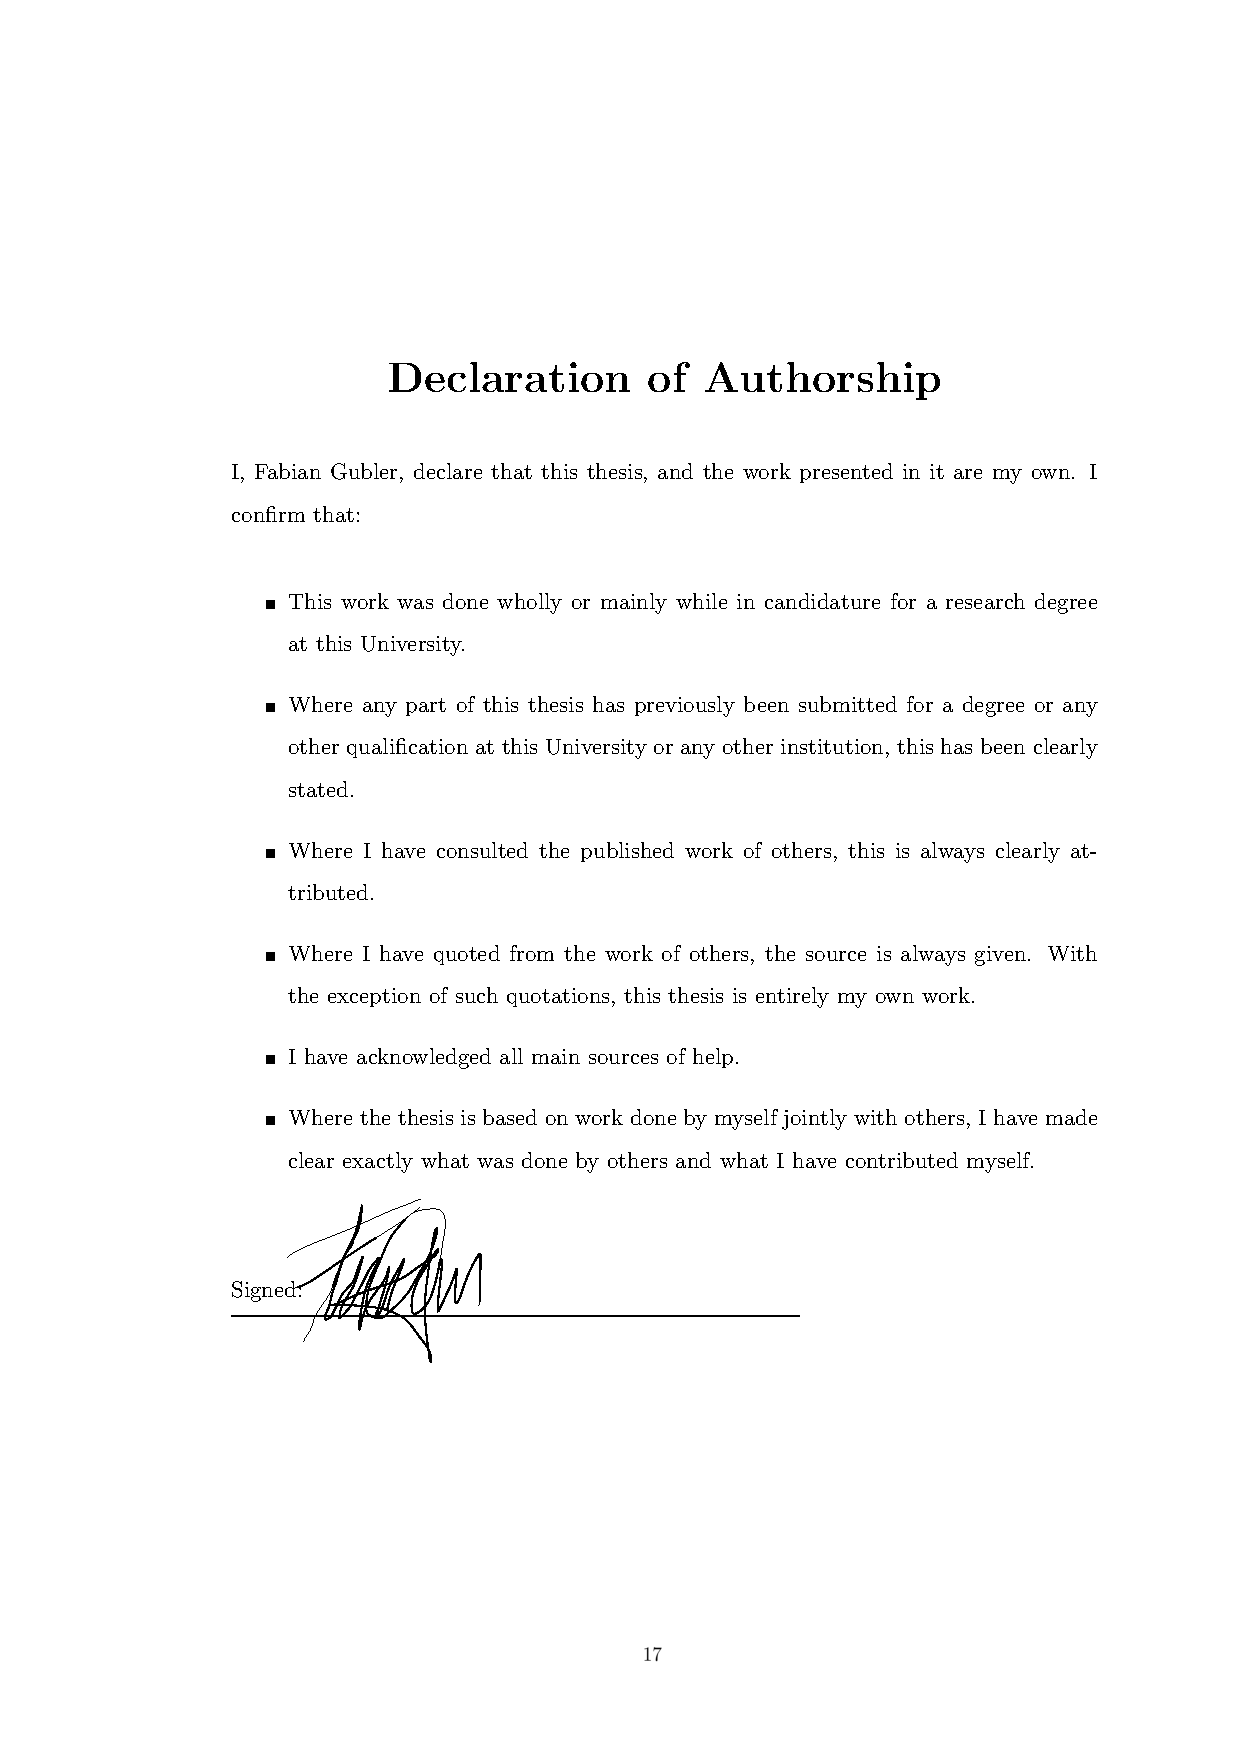
\includepdf[pages=-, offset=75 -75]{signed.pdf}
%% ----------------------------------------------------------------
% Declaration Page required for the Thesis, your institution may give you a different text to place here
\Declaration{

\addtocontents{toc}{\vspace{1em}}  % Add a gap in the Contents, for aesthetics

I, AUTHOR NAME, declare that this thesis titled, `THESIS TITLE' and the work presented in it are my own. I confirm that:

\begin{itemize} 
\item[\tiny{$\blacksquare$}] This work was done wholly or mainly while in candidature for a research degree at this University.
 
\item[\tiny{$\blacksquare$}] Where any part of this thesis has previously been submitted for a degree or any other qualification at this University or any other institution, this has been clearly stated.
 
\item[\tiny{$\blacksquare$}] Where I have consulted the published work of others, this is always clearly attributed.
 
\item[\tiny{$\blacksquare$}] Where I have quoted from the work of others, the source is always given. With the exception of such quotations, this thesis is entirely my own work.
 
\item[\tiny{$\blacksquare$}] I have acknowledged all main sources of help.
 
\item[\tiny{$\blacksquare$}] Where the thesis is based on work done by myself jointly with others, I have made clear exactly what was done by others and what I have contributed myself.
\\
\end{itemize}
 
 
Signed:\\
\rule[1em]{25em}{0.5pt}  % This prints a line for the signature
 
Date:\\
\rule[1em]{25em}{0.5pt}  % This prints a line to write the date
}
\clearpage  % Declaration ended, now start a new page

%% ----------------------------------------------------------------



%% ----------------------------------------------------------------
% Now begin the Appendices, including them as separate files

\addtocontents{toc}{\vspace{2em}} % Add a gap in the Contents, for aesthetics

\appendix % Cue to tell LaTeX that the following 'chapters' are Appendices

\chapter{Appendix A}
\lhead{\emph{Appendix A}}  % Set the left side page header

Lorem Ipsum
	% Appendix Title

\chapter{Appendix B}
\lhead{\emph{Appendix B}}  % Set the left side page header
 % Appendix Title

% \input{Appendices/AppendixC} % Appendix Title

\addtocontents{toc}{\vspace{2em}}  % Add a gap in the Contents, for aesthetics
\backmatter

%% ----------------------------------------------------------------
\label{Bibliography}
\lhead{\emph{Bibliography}}  % Change the left side page header to "Bibliography"
\bibliographystyle{unsrtnat}  % Use the "unsrtnat" BibTeX style for formatting the Bibliography
\bibliography{Bibliography}  % The references (bibliography) information are stored in the file named "Bibliography.bib"

\end{document}  % The End
%% ----------------------------------------------------------------
